\chapter{扰动场作用下的热负荷分析}


% 在之前的研究中,研究者曾经用 GENRAY 相关代码将场线进行推测。

上一章中我们基于对抑制 ELM 的需要提出了扰动场之间互相耦合的优化方法,这一章中我们承接其探究是否优化后的扰动场是否能够一定程度上缓解\Hmode 面对的热负荷问题。本部分研究的重点在于利用扰动场的对热负荷分布的影响,探究能否通过控制外加扰动场来控制热负荷,如果可行,如何使得材料受热受到的损害最小。


如果粒子在刮削层中运动时不考虑场的横向方向上的输运,即不考虑碰撞的情况,则难以模拟打到偏滤器上的热负荷分布。通过考虑粒子流在前进过程中可能产生的横向碰撞,我们基于蒙特卡洛的思想引入粒子沿磁力线移动时会发生的横向漂移。
粒子沿磁力线运动,但是每过一段满足指数分布的随机步长便发生横向漂移,使得粒子在不同磁力线之间可能发生漂移,通过粒子的蒙特卡洛模拟,模拟粒子速度分布造成的不确定性,改写之前我写的确定性的 FLT 的程序。通过在一个边界磁面附近以均匀分布的种子为起点,计算打到偏滤器上各种负荷分布的计算。

\section{热分布的优化理论}
螺旋电流丝产生了三维不对称的磁扰动结构,从而有着

需要展平偏滤器的二维曲面到平面上看分布得是否平坦。

尽管前一章节中对边界局域模的抑制是主要的评判扰动场的函数,评估热分布 $h(x,y)$ 优劣的函数,暂时选用梯度绝对值的 $\mathrm{L}^1$ 范数作为品质因子的计量标准,作为给定扰动场对应的热负荷分布的。
\begin{equation}
    \operatorname{FoM} =  \iint |\nabla h(x,y)| \mathrm{d} x \mathrm{d} y
\end{equation}

\begin{figure}[htbp]
    \centering
    \subcaptionbox{基于蒙特卡洛的磁力线扩散算法产生锯齿状的磁力线}{%
    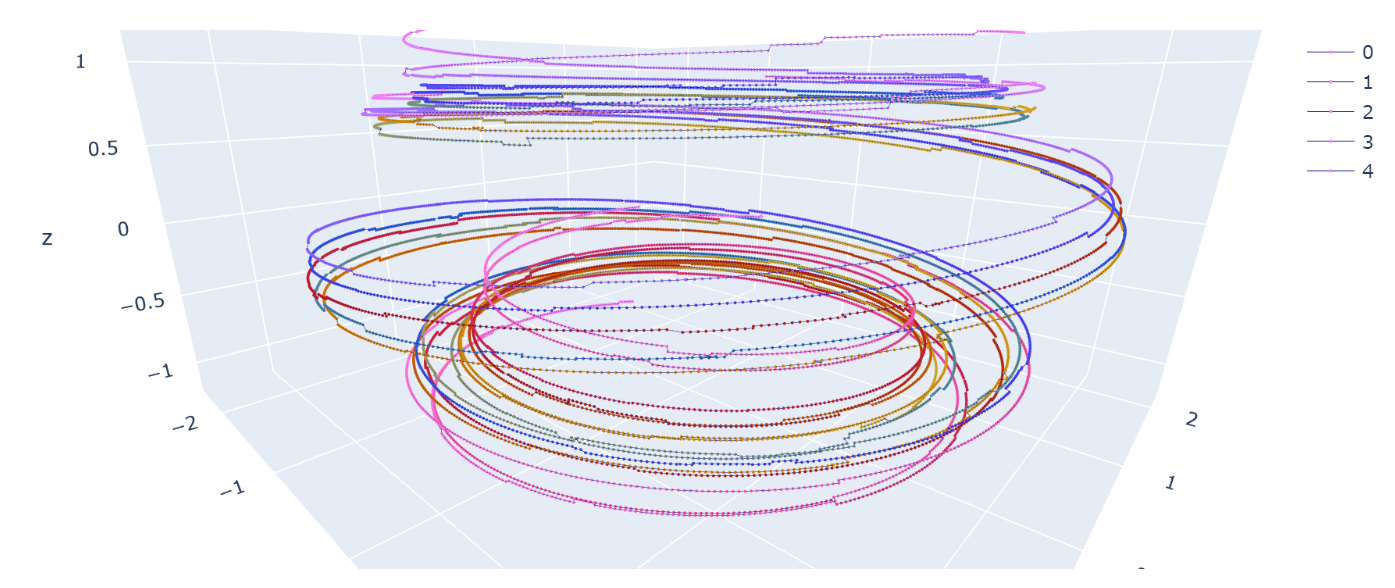
\includegraphics[width=0.85\columnwidth,keepaspectratio]{sawtooth_FLD.png}
    }%
\end{figure}


在粒子沿磁力线走过随机长度 $x$ 后发生一次横向漂移,
\begin{equation}
    p(x)=\frac{1}{\lambda} \exp \left(\frac{-x}{\lambda}\right)
\end{equation}

横向漂移的方向在垂直于场的平面内随机均匀分布,而步长则在下面区间是均匀随机分布的,
% The direction of the steps is uniform in the plane perpendicular to the field, while the step size $r$ is uniform in the interval:

\begin{equation}
    r \in[0, \sqrt{\frac{12 D_{\perp} \lambda}{v}}]
\end{equation}

该方法已在 Wendelstein 7-X 上成功应用以预估热负荷分布。

\section{扰动场作用下的热负荷分布调整}

\subsection{单个扰动场造成的热负荷分布特征}

\subsection{扰动场协同造成的热负荷分布特征}


\section{小结}

本节通过基于蒙特卡洛思想的磁力线扩散模拟了可能的热负荷在偏滤器平板上的分布。